\begin{center}

  \begin{tabular}{rp{16cm}lp{20cm}}%{rl}

  % after \\: \hline or \cline{col1-col2} \cline{col3-col4} ...

  论文地址:& \href{https://smcnus.comp.nus.edu.sg/wp-content/uploads/DGP.pdf}{https://smcnus.comp.nus.edu.sg/wp-content/uploads/DGP.pdf} \\

  %源码:& \href{xxx}{xxx} \\

  slides:& \href{https://smcnus.comp.nus.edu.sg/wp-content/uploads/DGP_slides.pdf}{{\footnotesize slides}}\\

  关键词:& \textbf{ASR, Relational Thinking, Deep Graph} \\

  写于:& \date{2020-12-10}

  \end{tabular}

\end{center}

该论文\cite{dgp}针对语音领域中如何对感知(percept)建模,并将感知融入到语音相关的问题中进行了探索,提出了一个贝叶斯非参数化的深度学习方法(Bayesian nonparametric deep learning method)--- Deep Graph random process(DGP),使用Graph对感知进行建模。

\paragraph{问题定义}
Relational Thinking是人类学习过程中至关重要的一个过程,在学习的过程中,我们会接收到各种各样的信息,不管是来自视觉、听觉、触觉等,但是我们并不会有意识地去保存它们(这是与Relational Reasoning的主要区别,relational reasoning是有意识地处理这些relation information)。在各种各样的信息之间隐藏着联系,这些信息及它们之间的联系组成了我们的percepts(感知)。论文针对语音/对话中信息之间隐藏的relation进行研究。

在通常的ASR(Automatic Speech Recognition)任务中,整个任务被分为两个过程:语音建模、语言解码,即以模式匹配的方法来解决这个问题。这种方法有一个很明显的缺点:没有考虑relational information,当然,如何将relational thinking融入到ASR中是很困难的。\tbc{red}{在交谈过程中,我们形成的感知是无意识的、无穷的}。有一些研究已经表明,在问答系统中,即使只将前一段对话的内容考虑到语音模型中,也会大大地提高模型的效果。但\tbc{red}{对percepts进行建模是很困难的} --- 这也是论文重点解决的问题。

目前,混合的语音循环神经网络隐马尔可夫模型(RNN-HMM)在许多方面仍优于端到端的编码-解码的方法,而且也越来越流行。RNN确实能够捕捉时间上的依赖关系,但对于复杂的关系(如relational thinking)则表现得不足。Graph能够描述更复杂的关系。但是依然存在一些挑战:
\begin{itemize}
	\item Graph相关的方法通常要求输入的数据是Graph形式的数据。但是在语音中并没有直接的图数据
	\item 目的是对relational thinking进行建模。但是在语音中percepts是隐含的
\end{itemize}


\paragraph{DGP 思路}DGP将relational thinking中的percepts建模为概率图,并且不需要任何关系数据。接下来更具体地描述DGP是如何对percepts进行建模的。

在语音中,处理的基本单位可以是音频数据的一个采样点、语音帧、语音片段(utterance)、一段语音等。论文中考虑的utterance,一个utterance可以是一句话的发音。在DGP中,给定一个utterance以及它之前的utterances(即历史utterances),可以生成无数个percept graphs,这与之前说到的relational thinking是相对应的。当前utterance和历史utterances之间不同的连接关可以看作一个percept(也许这就是它们称作\tbc{red}{percept graphs}的原因吧。以utterances连接成的Graph来定义percept)。为什么是无数个percept grpah呢?可以从直觉上来理解,在我们接收信息时,信息之间并没有生成稳定的信息,各个信息之间都是会产生关联的,并且基于我们的先验知识和历史信息,会在脑海中产生各种各样的理解 --- 相当于接收到的信息的不同组合,而这个组合是有无限可能的。并且,由于这些percepts是无意识的,percept graph中边的概率是接近于0的。

在DGP的percept graph中,Graph中的结点表示utterance,边表示结点之间的关系。论文中假设边的取值都服从Bernuli分布,且边的取值(即边存在的概率)是趋近于0的。看到这里貌似解决了对percepts建模的问题,但是该怎么解决涉及无数个percept graphs的问题呢?论文中对无数个percept graphs进行了transform,在percept graphs的基础上生成\tbc{red}{summary graph}。获得summary graph后即可将graph embedding作为语音模型的额外输入来提高模型性能。那么如何操作呢?

\paragraph{实现细节}
先定义一些形式化的表示。$U_i$表示utterance $i$,$U_{i-o:i-1}$表示$U_i$之前的$o$个utterances。$U_i$的特征是一系列的语音特征$\boldsymbol{X}_i = \{\boldsymbol{x}_{i,1}, \boldsymbol{x}_{i,2}, ... ,\boldsymbol{x}_{i,T}\}$,对应的标签为$\boldsymbol{Y}_i = \{\boldsymbol{y}_{i,1}, \boldsymbol{y}_{i,2}, ... , \boldsymbol{y}_{i,T}\}$。$\{ \alpha_{i,j}^{(k)} \}_{k=1}^{+\infty}$表示第$k$个percept graph中$U_i, U_j$间边存在的概率。$\{U_i\}_{i=1}^{M}$是用于训练模型的$M$个utterances。
\subparagraph{Deep Graph Random Process}
Deep Graph Random Process是一个随机过程,描述了一个机制,该机制主导无穷个概率图生成 --- 即无穷个percept graphs的生成。在percept graph中,每个结点是utterance的embedding:
$$
\boldsymbol{v}_i = f_{\theta}(\boldsymbol{X}_i)
$$
其中$f_{\theta}$是NN(Neural Network)。
DGP的核心是一系列的深度Bernuli过程(DBP),每一个DBP负责一对结点间边的生成,即:
$$
\{ \alpha_{i,j}^{(k)} \}_{k=1}^{+\infty} \sim DBP(Bern(\lambda_{i,j}))
$$
其中$Bern(\lambda_{i,j})$表示结点$i,j$间服从概率为$\lambda_{i,j}$的Bernuli分布,所有的percept graphs的边的概率都是从对应的Bernuli分布中采样的!

\subparagraph{Coupling of Innumerable Percept Graphs}
这一步的目的是如何生成summary graph,因为summary graph本身也是probablistic graph,而且结点已知,那么只剩节点之间边的概率了。其实从上一步就可以看出,单个percepet graph中边是服从Bernuli分布的,单考虑一条边的话,summary graph中对应边就是重复的Bernuli抽样,所以可以把summary graph中的边看作是服从Binomial分布的。那么summary graph中边的概率为:
$$
\tilde{ \alpha}_{i,j} = \sum_{k=1}^{+\infty} \alpha_{i,j}^{(k)},\;\; \tilde{ \alpha}_{i,j} \sim \mathcal{B}(n, \lambda_{i,j})
$$
但上式存在一个问题,$n \rightarrow +\infty,\; \lambda_{i,j} \rightarrow 0$,那么该如何解决这个问题呢?

\subparagraph{Inference and Sampling of Edges of Summary Graph}
为了采样得到summary graph中边的概率,论文中采用一个高斯分布来近似上文提到的Binomial分布。对于每条边,近似的高斯分布为:
$$
\mathcal{N}(m_{i,j}, m_{i,j}(1-m_{i,j})),\;\; m_{i,j} = n\lambda_{i,j}
$$

\subparagraph{Application of DGP for Acoustic Modelling}
为了从summary graph中提取出更具有代表性的信息,或者说为了更好地适应下游的任务,还需要对summary graph进行一个转换。转换的方式是赋予每条边一个权重,生成新的图 --- \textit{task-specific graph}(\tbc{red}{这样做的原理论文中并没有给出})。这很像注意力机制。权重是从一个高斯分布中采样得到的,那么task-specific graph的边表示为:
$$
\overline{ \alpha}_{i,j} = s_{i,j} * \tilde{ \alpha}_{i,j}
$$
上式中$s_{i,j}$是对应边的权重,论文中对权重服从的高斯分布进行了一定的假设:权重是以summary graph边的取值为条件的,即:
$$
s_{i,j}|\tilde{ \alpha}_{i,j} \sim \mathcal{N}(\tilde{ \alpha}_{i,j} * \mu_{i,j}, \tilde{ \alpha}_{i,j} * \sigma_{i,j}^2)
$$
得到task-specific graph后,即可按照GNN/GCN的方式获得graph embedding(注意:每处理一个utterance时都会有对应的task-specific graph)。接下来就是应用上述一系列工作的结果 --- graph embedding了。论文中将整个框架称作 relational thinking network(RTN),使用simple recurrent unit(SRU)作为构建单元。具体的可以参考SRU,说明一下如何在acoustic model中使用graph embedding:将graph embedding与原来的输入进行拼接即可。

\subparagraph{Learning}
知道了上述步骤,那么如何来学习整个模型呢?论文中使用variational inference来联合训练DGP、task-specific graph中边的权重、acoustic model。这个可以参考\cite{kingma2014autoencoding},目标函数是evidence lower bound(ELBO):
\begin{equation}\nonumber
	\begin{array}{l}
		\sum_{i=1}^{M}\left\{\mathrm{KL}\left(q\left(\tilde{\mathbf{A}}, \mathbf{S} \mid \mathbf{X}_{i-o: i}\right) \| p\left(\tilde{\mathbf{A}}, \mathbf{S} \mid \mathbf{X}_{i-o: i}\right)\right)\right. \\
		\left.\quad-\mathbb{E}_{\tilde{\mathbf{A}}, \mathbf{S}}\left[\log P\left(\mathbf{Y}_{i} \mid \mathbf{X}_{i}, \tilde{\mathbf{A}}, \mathbf{S}\right)\right]\right\}
	\end{array}
\end{equation}
其中,$\tilde{\mathbf{A}} = [\tilde{ \alpha}_{i,j}],\;\; \mathbf{S} = [s_{i,j}]$。上式可以转化为:
\begin{equation}\nonumber
	\begin{aligned}
		\sum_{(i, j) \in \tilde{E}}\{& \mathrm{KL}\left(\mathcal{B}\left(n, \tilde{\lambda}_{i, j}\right) \| \mathcal{B}\left(n, \tilde{\lambda}_{i, j}^{(0)}\right)\right.\\
		&+\mathbb{E}_{\tilde{\alpha}_{i, j}}\left[\mathrm{KL}\left(\mathcal{N}\left(\tilde{\alpha}_{i, j} \odot \mu_{i, j}, \tilde{\alpha}_{i, j} \odot \sigma_{i, j}^{2}\right)\right.\right.\\
		&\left.\left.\| \mathcal{N}\left(\tilde{\alpha}_{i, j} \odot \mu_{i, j}^{(0)}, \tilde{\alpha}_{i, j} \odot \sigma_{i, j}^{(0)^{2}}\right)\right]\right\}
	\end{aligned}
\end{equation}
但并不能直接最大化上式来作为优化目标,因为其中会涉及到$n \rightarrow +\infty$,所以还需要对其进行转化,具体的转化过程可以参考论文中的证明和附带材料。

Okay,整个过程就是这样了,整体框架如Fig.\ref{fig:dgp}所示。论文中还对RTN的具体实现进行了介绍,包括上文中涉及到的一些参数的计算,如$m_{i,j}, \mu_{i, j}, \sigma_{i, j}$等,以及模型的网络结构等。
\begin{figure}[h]
	\centering
	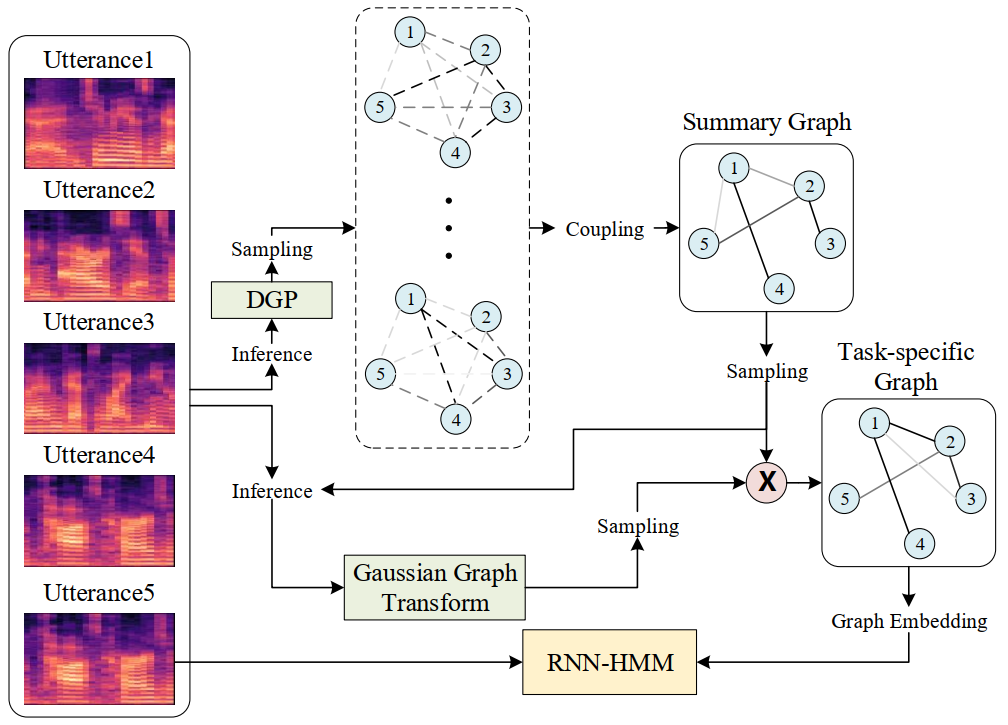
\includegraphics[width=.8\textwidth]{pics/dgp.PNG}
	\caption{Architecture of RTN for acoustic modelling}
	\label{fig:dgp}
\end{figure}

\paragraph{方法解决的问题/优势}

\begin{itemize}
	\item 提出了一种对percept建模的方法,percept graphs的想法很棒
	\item 以graph的形式表示percepts,并无需relation data就可以学习到隐含的relational thinking
	\item 将relational thinking融入到acoustic model中
\end{itemize}



\paragraph{方法的局限性/未来方向}
\begin{itemize}
	\item 个人认为variational inference会涉及到较多的运算
	\item \tbc{red}{可以将percept graphs的想法应用到更多的问题上}
	\item task-specific graph的由来没有解释清楚	
	\item \tbc{red}{论文中只结合了历史的utterances,并没有结合先验知识}。尽管不同的人先验知识是不同的,但是在某个特定的应用场景下,先验知识是有范围的,可以借助知识图谱来表示先验知识,再结合本文的方法完成特定场景下的对话任务。\tbc{red}{这也可以看作是一个多模态信息融合的方法}
	\item 在生成summary graph时,相当于给所有的percept graphs分配了相等的权重(注意力),然而在实际的思考过程中,\tbc{red}{不同的percepts应该有不同权重的,在生成summary graph时对不同的percept graphs赋予不同的注意力是否更合理?
	}

\end{itemize}
